\documentclass[border=10pt]{standalone}
\usepackage[svgnames]{xcolor}
\usepackage{amsmath}
\usepackage{pgfplots}
\pgfplotsset{compat=newest}
\usepackage[sfdefault]{FiraSans}
\usepackage{FiraMono}
\renewcommand*\familydefault{\sfdefault}
\begin{document}
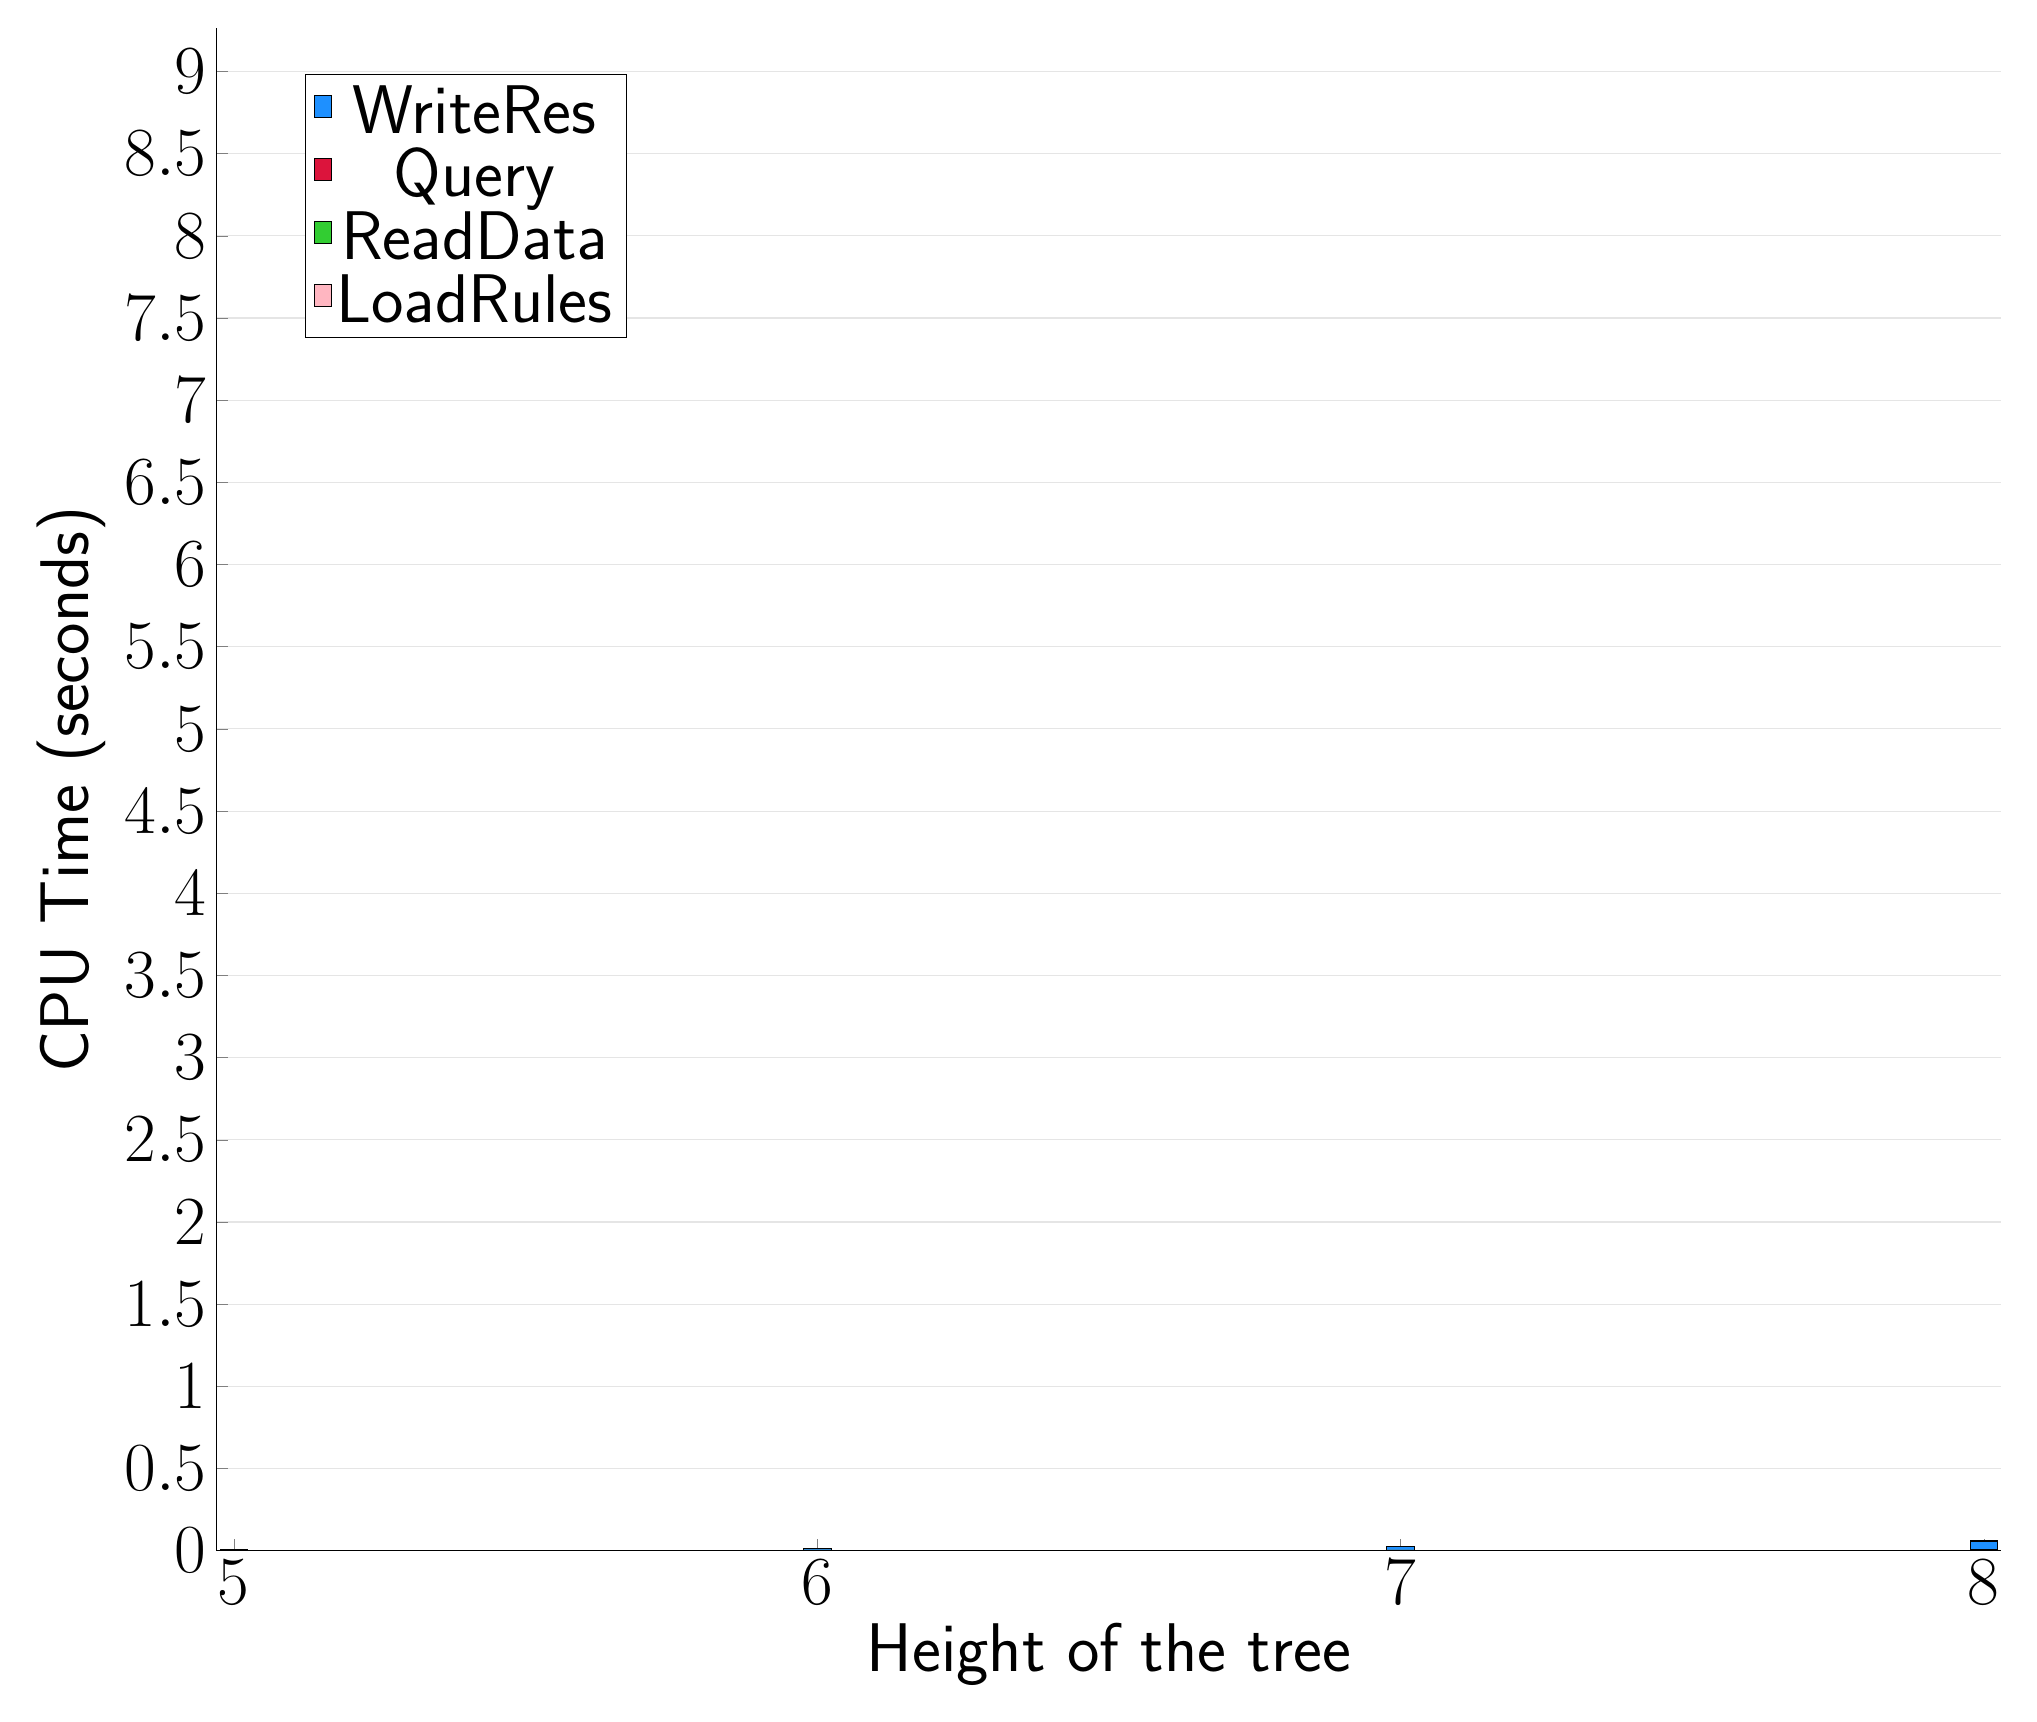
\begin{tikzpicture}
\begin{axis}[
   ybar stacked,
   width=2\textwidth,
   bar width=0.35cm,
   ymajorgrids, tick align=inside,
   major grid style={draw=gray!20},
   xtick=data,
   ymin=0, ymax=9.263333335518837,
   axis x line*=bottom,
   axis y line*=left,
   enlarge x limits=0.01,
   legend style={
       at={(0.23, 0.97)},
       anchor=north east,
       legend columns=1,
       font=\Huge,
   },
   ylabel={CPU Time (seconds)},
   xlabel={Height of the tree},
   label style={font=\Huge},
   tick label style={font=\Huge},
]
\addlegendimage{fill=DodgerBlue, draw=black, line width=0.2pt}
\addlegendentry{WriteRes}
\addlegendimage{fill=Crimson, draw=black, line width=0.2pt}
\addlegendentry{Query}
\addlegendimage{fill=LimeGreen, draw=black, line width=0.2pt}
\addlegendentry{ReadData}
\addlegendimage{fill=LightPink, draw=black, line width=0.2pt}
\addlegendentry{LoadRules}
\addplot +[fill=LightPink, draw=black, line width=0.2pt] coordinates {
(5, 0.0024403333333333334)
(6, 0.0033583333333333334)
(7, 0.0028820000000000004)
(7, 0.003137000000000003)
(7, 0.002713)
(8, 0.0029806666666666666)
(8, 0.003885000000000003)
(8, 0.00115)
};
\addplot +[fill=LimeGreen, draw=black, line width=0.2pt] coordinates {
(5, 0.0008856666666666657)
(6, 0.0013579999999999998)
(7, 0.0018166666666666635)
(7, 0.002130333333333333)
(7, 0.0020650000000000004)
(8, 0.0037476666666666665)
(8, 0.003941)
(8, 0.0010783333333333333)
};
\addplot +[fill=Crimson, draw=black, line width=0.2pt] coordinates {
(5, 3.5333333333333966e-05)
(6, 7.133333333333067e-05)
(7, 0.00013533333333333103)
(7, 0.00015733333333333536)
(7, 0.00017466666666666433)
(8, 0.000392666666666666)
(8, 0.0004003333333333313)
(8, 0.00010599999999999966)
};
\addplot +[fill=DodgerBlue, draw=black, line width=0.2pt] coordinates {
(5, 0.003999333333333333)
(6, 0.009337333333333336)
(7, 0.02185266666666667)
(7, 0.02105)
(7, 0.020775000000000002)
(8, 0.05402766666666667)
(8, 0.05292933333333333)
(8, 0.054073)
};
\end{axis}
\end{tikzpicture}

\end{document}
